%
% Szakdolgozatminta az Eszterházy Károly Katolikus Egyetem
% matematika illetve informatika szakos hallgatóinak.
%

\documentclass[
% opciók nélkül: egyoldalas nyomtatás, elektronikus verzió
% twoside,     % kétoldalas nyomtatás
% tocnopagenum,% oldalszámozás a tartalomjegyzék után kezdődik
]{thesis-ekf}
\usepackage[T1]{fontenc}
\usepackage{hulipsum}
\PassOptionsToPackage{defaults=hu-min}{magyar.ldf}
\usepackage[magyar]{babel}
\usepackage{mathtools,amssymb,amsthm,pdfpages}
\footnotestyle{rule=fourth}

\newtheorem{tetel}{Tétel}[chapter]
\theoremstyle{definition}
\newtheorem{definicio}[tetel]{Definíció}
\theoremstyle{remark}
\newtheorem{megjegyzes}[tetel]{Megjegyzés}


\begin{document}
	\institute{Matematikai és Informatikai Intézet}
	\title{Programozható elektronikák alkalmazásai}
	\author{Bagoly Gábor\\Programtervező informatikus}
	\supervisor{Dr. Geda Gábor\\Egyetemi docens}
	\city{Eger}
	\date{2023}
	\maketitle
	\tableofcontents
	
	\chapter*{Bevezetés}
	\addcontentsline{toc}{chapter}{Bevezetés}
	
	Mai világunkban az okos otthonok és az okos eszközök rendkívül népszerűek és elterjedtek lettek. Általában, hogy ha megkérdezünk valakit ezzel a témával kapcsolatban, akkor nagy valószínűséggel azt tudják mondani, hogy rendelkeznek legalább egy okos otthonban alkalmazható eszközzel. Ezek az eszközök lehetővé tehetik a kényelmesebb és hatékonyabb életmódot. 
	
	De mi is tesz egy eszközt okossá? Feltételezhetjük azt, hogy ha valamelyik eszköz internetre kapcsolódik, esetleg távolról beállíthatjuk, vagy automatizálhatjuk előre meghatározott dolgokra, akkor azt az eszközt ,,okosnak'' tudjuk mondani.
	
	Hogy ha valaki már rendelkezik több ilyen eszközzel, akkor bizonyára találkoztak már azzal a problémával, hogy egy bizonyos ökoszisztémában használatos eszköz nem feltétlenül tud működni egy másikban. Minderre próbáltam egy olyan megoldást kitalálni, ami abból a szempontból közelíti meg mindezt, hogy még egy 'nem okos' eszközt (például egy izzót) integrálok bele úgy a rendszerbe, hogy azt egyszerűen tudjunk kezelni bárhonnan az otthonunkból, ehhez társulva különböző programozható elektronikák. Mindehhez egy olyan rendszert hoztam létre, amelynek a háttérben lévő folyamatok lebonyolítását egy webes alkalmazás végzi el, és az általunk ismert legtöbb eszközön használható, amin internetezni is tudunk: legyen az számítógép, Androidos, vagy iOS-es telefon, tablet, vagy akár okos óra is.
	
	Azért került erre a témára a választásom, mivel számomra felettébb érdekes az, hogy egy ilyen okos otthonban az eszközök hogyan is kommunikálnak, és szeretnék ebbe egy belátást nyerni, hogy hogyan is épül össze mindez.

	Célom az lenne ezzel, hogy belelássak egy ilyen rendszer működésébe, különböző programozható eszközök alkalmazását jobban megismerjem, és, hogy egy olyan általános kezelőfelületet tudjak létrehozni, amit könnyen tud a felhasználó alkalmazni.
	
	\chapter{Piacon lévő jelentősebb okos otthon rendszerek}
	\section{Nagyobb cégek által létrehozott ökoszisztémák}
	Amikor arra jut a sor, hogy okos otthont szeretnénk összeállítani, akkor ahhoz egy széles palettából tudunk választani eszközöket, legyen az biztonsági kamera, ajtózár vagy akár háztartási eszközök, mint például egy mosógép vagy robot porszívó. Amikor az okos otthon rendszer kiválasztására kerül sor, fontos figyelembe venni az ehhez alkalmazandó eszközök kiválasztását is.
	
	Van néhány olyan eszköz, -- például az okos izzók -- amelyek szerencsére több okos otthon rendszerben is könnyen alkalmazhatóak. Ezek az eszközök általában ipari szabványokat használnak, mint például a Zigbee\footnote{Zigbee-t használ például az Amazon Echo, a Google, az IKEA okos otthon termékei, és a Philips Hue}, ami lehetővé teszi számukra, hogy működjenek a különböző okos otthon rendszerekkel. 
	
	Azonban vannak olyan eszközök is, amelyek csak egyetlen rendszerrel használhatóak. Ezek az eszközök saját szabványokat alkalmaznak, amelyek nem kompatibilisek más rendszerekkel. Vegyük például azt, hogy ha egy olyan okos eszközt veszünk, ami csak egy meghatározott okos otthon rendszerrel működik együtt, akkor az eszközt később nem tudjuk használni egy másik rendszerben.
	
	Mindezek alapján amikor okos eszközt vásárlunk, akkor nagyon oda kell figyelni, hogy kompatibilis-e a választott okos otthon rendszerünkkel, amit általában fel szoktak tüntetni az eszközök leírásában, vagy, hogy ha utána keresünk mindennek.
			
	\subsection{Mik is a virtuális asszisztensek?}
	A virtuális asszisztensek olyan szoftveres programok, amik különböző feladatokat tudnak elvégezni felhasználó kérésére. Ezek persze mindezeknek korlátjainak megfelelően.
	
	Úgy lettek megalkotva, hogy a felhasználó hang vagy esetleg chat alapon tudjanak egyszerű kérdéseken keresztül kommunikálni vagy utasításokat adni. A virtuális asszisztensek olyan feladatokban tudnak segíteni, mint emlékeztetők létrehozása, üzenetek küldése, hívások indítása, interneten való keresés, időjárás előrejelzések felolvasása, okos otthoni eszközök irányítása, és egyéb más dolgok. 
	
	Számos cég hozott már létre magának virtuális asszisztenst, amik közül a legismertebbek lehetnek a Google által létrehozott Google Asszisztens, Apple-nek Siri, Amazon-nak Alexa, Samsung Bixby-je, és Microsoft Cortana-ja.
	
	Hogy ha például egy újabb Samsung telefonja van az embernek, akkor azon két virtuális asszisztens is jelen van (Google Assistant és Bixby), de letölthető akár mellé harmadiknak az Amazon Alexa is.
	
	\subsection{Amazon rendszere - Alexa Smart Home}
	2014-ben lépett be be a piacra az Amazon -- \emph{az akkor még újdonságnak számító} -- okos hangszórójukkal, az Amazon Echo-val. Ekkor még leginkább csak annyira volt képes, hogy a felhasználó zenét tudja irányítani hang utasításokkal. Ez az eszköz úgy működik, hogy ebbe bele van integrálva az Amazon sajátos virtuális asszisztense, amit Alexának hívnak. Ugye mint kezdetleges szoftver, neki sem voltak a képességei túl szerteágazóak. Leginkább arra tudta az ember használni, hogy egyszerű kérdéseket tegyen fel az ember, és zenét tudjon elindítani, leállítani átugrani.
	
	Nem is annyira később, amikor elkezdett egyre jobban fejlődni Alexa, úgy egyre több mindenre kezdhette el használni az ember: termosztátok beállítása, izzók ki- és bekapcsolására is már lehetett használni. Miután az Amazon egyre többet fektetett bele a rendszerükbe felettébb szerteágazó lett annak a használata az otthonokban. Még arra is volt lehetőség már ekkor, hogy akár bevásárló listát készítsen, és azokat meg is tudja rendelni a felhasználó az Amazonról, mindezt Alexa használatával. A cég 2017 május 23-án jelentette be, hogy a \emph{Smart Home Skill API}-jukba\footnote{A blog poszt amiben bejelentették a Smart Home Skill API bővítését\cite{amazon-api}} innentől kezdve megadható, hogy milyen eszközöket is csatlakoztatunk a rendszerükbe, ami kitárta a lehetőségeket az otthoni okos készülékek automatizációjára. Mindez vezetett az okos otthon piac és a virtuális asszisztensek szerepének növekedéséhez.
	
	Eszközök leginkább hangvezérléssel irányíthatóak, miután követtük az általuk biztosított használati útmutatót. Néhány esetben az Amazon Alexa alkalmazás elegendő lehet, de ha olyan eszközt szeretnénk használni, amelyhez saját alkalmazás tartozik, akkor azt is le kell töltenünk.
	
	Az Amazon által szolgáltatott okos otthon rendszer 2023-ra olyan népszerűségi szintre jutott, hogy az Amerikai Egyesült Államokban az ilyen hang vezérelt hangszórók 68.2\%-a az Amazon Echo.\footnote{Statisztikai adatokat az Earthweb: ,,How Many People Use Alexa in 2023? (U.S. Amazon Statistics)'' cikkjéből \cite{amazon-stats}} 
	
	Mindezzel napjainkban több ezer eszköz használható már ezen a rendszeren belül: legyen az biztonsági rendszer, háztartási gépek, vagy esetleg szórakoztató rendszerek. Érthető is, hogy sokan miért is szeretik ezt a rendszert használni.
	
	Azonban ennek a rendszernek is megvannak azok a hátulütői, mint például az, hogy nem tudunk felhasználni benne olyan eszközöket, amik nem támogatottak az Amazon által. Érdemes arra odafigyelni, hogy amikor egy okos eszközt veszünk, hogy arra fel-e van tüntetve, hogy kompatibilis az Amazon rendszerével. Másik ilyen negatív tényező lehet számunkra az is, hogy az Amazon Alexa nem használható magyar nyelven még.
	
	\subsection{Google rendszere - Google Home és Google Nest}
	Az Amazon Echo sikere után a Google is részesülni akart az okos otthon piacának sikereivel. 
	
	Az akkor még Nest Labs által készült termékek olyanok voltak mint az öntanuló termosztát -- amit 2011-ben hoztak létre ,,Nest Learning Thermostat''\footnote{Magyarul: Nest Tanuló Termosztát} néven, ami Wi-Fi-re kapcsolható volt, és szenzorok segítségével alkalmazkodhatott a beltéri hőmérsékleti körülményekre. Ezt követte a következő termékük, a füst és szén-monoxid érzékelő, aminek a neve ,,Nest Protect'' volt. 2014-ben felvásárolták a Dropcam nevezetű céget ami biztonsági kamerákat készítettek, amik után a Nest Labs ezt követő terméke a Nest Cam volt 2015-ben.
	
	A Nest Labs egyre jobban látszódó sikerének köszönhetően a Google felvásárolta 2014 januárjában. 2018-ig még önállóan működött a Nest, ami után beolvasztották a Google otthoni termékcsaládba, ezzel létre hozva a Google Nest termékcsaládot, ami számos termékekkel rendelkezik mostanára: termosztát, ajtócsengő, ajtózár, biztonsági kamera, virtuális asszisztenssel integrált érintőképernyős központi egység.\footnote{\label{google-store} További jelenleg elérhető Google Nest családba tartozó termékek: \url{https://store.google.com/gb/category/connected_home} oldalon megtalálható}
	
	Az Amazon Echo-hoz hasonló első terméke a Google-nek a Google Home volt, amit 2016 októberében jelentettek be. Ez a cég sajátos virtuális asszisztensével a Google Assistant-tel volt felszerelve, és ugyan úgy lehetett neki utasításokat adni, és kérdéseket feltenni. Azóta már több otthonon belül alkalmazható eszköz elérhető egyenesen a Google Store-ból.\footref{google-store} Vagy egyéb támogatott harmadik felek által készített ilyen eszközökkel.
	
	Az egyik legnagyobb előnye a Google Home rendszernek az integrációja más Google szolgáltatásokkal, mint például a Google Térkép, a Google Naptár és a Google Fotók. Ez azt jelenti, hogy a felhasználók kéz nélkül is hozzáférhetnek személyes információikhoz és ütemtervükhöz, szimplán csak a Google Asszisztensnek feltéve a kérdést.
	
	A Google Home rendszer másik erőssége az, hogy képes felismerni a különböző hangokat, amely lehetővé teszi a személyre szabott válaszokat és információkat minden háztartási tag számára. Ez különösen hasznos lehet több személyes háztartásokban, ahol több ember is használja a rendszert.\footnote{Erre ugyan úgy betanítható az Amazon Alexa is.}
	
 	Mindezek által a Google Home rendszer erős versenytárs az okos otthon piacon.
	
	Viszont a Google Home-nak is meg vannak azok a hátrányai mint az Amazon rendszerének. Sajnos inkább csak akkor tudjuk kihasználni ennek a rendszernek az előnyét, ha angolul vagy más támogatott nyelven beszélünk vele, amibe még nem tartozik bele a magyar.
	
	\subsection{Xiaomi rendszere - Mi Home}
	A Xiaomi 2015 júniusában dobta piacra első okos otthon termékcsomagját, a ,,Smart Home Kit''-et, amely mozgásérzékelőt, lámpát és kapacitív kapcsolót tartalmazott. Ezeket az eszközöket egy alkalmazás segítségével lehetett vezérelni, ami lehetővé tette a felhasználók számára, hogy különböző utasításokat állítsanak be, például hogy a mozgásérzékelő észlelésekor a lámpa felkapcsoljon, vagy értesítést küldjön a felhasználónak, illetve a csomag támogatta a Xiaomi biztonsági kameráját is. \cite{xiaomi-home}
	
	Ma a Xiaomi okos otthon termékpalettája rendkívül sokrétű, a forrólevegős sütőktől, a robotporszívókon, és a szobamérlegeken át a hőmérséklet- és páratartalom-szenzorokig. Az összes termékük integrálható a Mi Home alkalmazásba, és a felhasználók harmadik féltől származó eszközöket is csatlakoztathatnak hozzájuk.
	
	Nagy előnye a Xiaomi okos otthon termékeknek az, hogy viszonylag olcsóbb a konkurens termékektől, és fel is használható például a Google Home, és az Amazon Alexa Smart Home rendszeren belül is, és használata felettébb felhasználó barát.
	
	Kisebb hátránya lehet neki az, hogy ezeket az eszközöket nem lehet asztali alkalmazáson keresztül irányítani, csak is az Androidos és iOS-es alkalmazáson keresztül, vagy esetleg a Google Home vagy Alexa Smart Home-on belül. Amazon Alexával a párosítás mostanában sajnos nehézkesebb, mivel valamilyen oknál fogva nagy százalékban nem tud csatlakozni valami hibánál fogva. Még olyan is megesik, hogy nem minden eszköz érhető el például a Google Home felületen, ilyen lehet példának a biztonsági kamerájuk, ami csak a saját alkalmazásukon érhető el. És mint az előző kettő rendszernél, ez sem használható még magyar nyelven.
	
	\section{Nyílt forráskódú rendszerek}
	\subsection{Mit is az, hogy open source?}
	Open source, azaz nyílt forráskódú szoftver az olyan, aminek a forráskódját szabadon lehet vizsgálni, módosítani, és akár ki is egészíteni. A kód az a része egy szoftvernek amit a legtöbb felhasználó bizonyára soha nem fog látni. Ez az a kód, amit a programozók változtathatnak hogy megváltozzon a program vagy alkalmazás működése. Azok a programozók, akik hozzáférhetnek egy szoftver forráskódjához, azokat feljeszthetik, és javíthatják azzal hogy például új funkciót adnak hozzá, vagy kijavítanak egy olyan részt, ami nem minden esetben működik helyesen.\footnote{\label{open-source-fn}A nyílt forráskódú szoftverről az irodalomjegyzék \cite{what-is-open-source}. részén található}
	
	Azonban azt, hogy egy szoftver nyílt forráskódú, nem feltétlenül jelenti azt, hogy az adott szoftver ingyenes használatban áll. Nyílt forráskódot fejlesztő programozók kérhetnek pénzt azért a nyílt forrású szoftverért, hogy ha ők alkották meg, vagy hozzájárulásukkal készült el. 
	
	Bizonyos esetekben azonban, mivel a nyílt forráskódú licenc megkövetelheti a program forráskódjának kiadását amikor szoftvert adnak el másoknak, egyes programozók úgy találják, hogy jövedelmezőbb pénzt kérni a felhasználóktól a szoftverszolgáltatásokért és - támogatásért (nem feltétlenül magáért a szoftverért). Így a szoftvereik ingyenesek maradnak, és pénzt keresnek azzal, hogy másoknak segítenek telepíteni, használni és hibaelhárítást végezni.\footref{open-source-fn}
	
	\subsection{Home Assistant}
	A Home Assistant 2013 novemberére került publikálásra \emph{GitHub.com}-on \textsc{Paulus Schoutsen} által. Ez ekkor még egy Python programozási nyelven megírt alkalmazás volt.
	Ekkor még ez egy egyszerű program volt, ami napnyugtakor felkapcsolta a lámpát. Azóta a szoftver elég érett lett, és körülbelül 20 aktív hozzájáruló dolgozik a projekten, ennek köszönhetően kéthetente érkezik frissítés a rendszerre.\footnote{\label{history-of-home-assistant}A történet bővebben az irodalomjegyzék  \cite{creation-of-home-assistant}. részén megtalálható.}
	
	Ez a szoftver bármely olyan rendszeren működik, ami a Python 3 programozási nyelvet tudja futtatni. Biztosít mobil és számítógép alkalmazást is, mellyel több ezer támogatott eszközt tudunk irányítani. Annyi a különbség ez a rendszer és a nagyobb cégek által biztosított között, hogy ez teljesen lokálisan fut, és hogy ha esetleg internet kimaradás lenne, még akkor is tudjuk ugyan úgy irányítani eszközeinket. A rendszer által számos ismert okos eszköz támogatott, mint például a Philips Hue, IKEA TRÅDFRI, és akár az Amazon Echo, Google Home, és a Xiaomi Mi Home által támogatott eszközök, és még a virtuális asszisztensük is.\footnote{A támogatott rendszerek a weboldalukon elérhető, ami az irodalomjegyzék \cite{home-assistance-itegrations}. részén megtalálható} Mindez annak köszönhető, mert Z-Wave és a Zigbee protokoll is támogatott a rendszer által, és mivel nyílt forráskódú a szoftver, ezért bármikor lehet az hogy valamelyik felhasználó vagy esetleg fejlesztő hozzáadja bizonyos termékeket kiegészítésként. 

	A rendszerrel háztartásunk energiafelhasználását is nyilván lehet tartani. Szabadon testre szabható a felület kinézete a felhasználók ízlése szerint. Szintén pozitívum lehet, hogy az szoftver támogatja a magyar nyelvet is.
	
	Ámbár ez a rendszer azoknak ajánlott jobban, akik informatika terén ismertek.
	
	\subsection{OpenHAB}
	
	OpenHAB, azaz Open Home Automation Bus\footnote{Magyarul: Nyílt Otthon Automatizációs Busz} fejlesztése 2010-ben kezdődött, és Java programozási nyelvben lett megírva. 2013-ban került elérhetővé az első stabil verziója a szoftvernek. 
	
	Az OpenHAB legelső körben azon a személyek számára ajánlott, akik jól ismertek informatika, és robotika terén. Ez azért szükséges, mert nekünk kell összeállítanunk, hogy mit szeretnénk elérni az okos otthon rendszerünkben. Az alkalmazás rendkívül rugalmas és testre szabható, és nagy a támogatottsága. Ez az egyik legelterjedtebb nyílt forráskódú okos otthon rendszer, és folyamatos fejlesztés alatt áll egy nonprofit szervezet által, aminek a fejlesztésébe bárki beállhat.
	
	Ez a rendszer képes integrálni a piac különböző eszközeit, mint ahogyan azt a Home Assitant rendszernél is említettem. Szintén egy fontos tényezője, hogy lokálisan működik, ezért egy internet kimaradásnál az okos otthonunk ugyan úgy működni fog. 
	
	A szoftvernek hivatalos oldalon megtalálható a teljes dokumentációja, hogy mit hogyan kell összeállítani és használni, ezért lehet kedvelt olyan személyek számára, akik szeretik a dolgokat maguknak összeállítani. A rendszer nagy támogatást és közösséget élvez, így ha felmerülne bármilyen kérdés, biztosan választ kapunk rá.
	
	Az ezzel létrehozott otthonunkat a legtöbb felületen el tudjuk érni, legyen az MacOS, Windows, Linux, Android vagy iOS.
	\footnote{Az OpenHAB hivatalos oldala megtalálható a az irodalomjegyzék \cite{openhab}. részén, ahol olvasható a dokumentációjuk, a céljaik, és egyéb blogjaik.}
	
	%----------
	\chapter{Alkalmazott eszközök}
	
	Ebben a fejezetben azt fogom taglalni, hogy milyen eszközöket is használtam az okos otthon rendszerem létrehozása során. Legyenek ezek hardveres vagy szoftveres komponensek. 
	
	Mindezek közben fogok csatolni kötési rajzokat, amik arra tesznek betekintést, hogy hogyan is kell összekötni ezeket az eszközöket, hogy a rendszerben működjenek.
	
	Szoftveres komponensek közé tartoznak azok a szoftverek, amik a projekt létrehozása közben fel voltak használva: legyen az keretrendszer, programozási nyelv, vagy stílus megírásra használt külső komponens.
	
	\section{Hardver}\label{hardware-sec}
	\subsection{Mi is az hogy IoT?}
	IoT\footnote{(Internet of Things) - magyarul: Internet dolgai}-k azok olyan eszközök, melyek Wi-Fi hálózaton keresztül párosíthatóak, és irányíthatóak. Ilyenek lehetnek a háztartásunkban levő olyan eszközök, melyeket távolról is tudunk irányítani interneten keresztül. Legyen ez például a Xiaomi forrólevegős sütője, vagy egy okos izzó. 
	
	Ebbe a kategóriába tartoznak a mikrokontrollerek is, amik mini programozható elektronikák, az alkalmazott Raspberry Pi 4B is.
	
	\subsection{Raspberry Pi 4B}
	A projektnek szíve-lelke egy bankkártya méretű mini számítógép, ami szolgáltatja a vezeték nélküli internetet az otthoni eszközök számára, ezzel megvalósítva a később említett programozható elektronikáknak is a kommunikációt.
	
	A Raspberry-n dolgozódnak fel az adatok, és ez általa szolgáltatott a webalkalmazás is. Felettébb sokoldalú a használata, és előszeretettel van használva okos otthon projektek megvalósításában is, például hogy ha Home Assistant-el, vagy OpenHAB-bal szeretnénk azt megvalósítani.
	
	Eben Upton 2012-ben hozta létre az első ilyen kis számítógépet, a Raspberry Pi 1 Model B-t. Raspberry magyarul azt jelenti, hogy málna mivel, ebben az időben többen is hoztak létre elektronikai termékeket gyümölcs nevekkel felruházva: legyen az Apple (alma), Acorn (makk), Apricot (sárgabarack).
	
	Elsődleges célja az volt Eben Upton-nak hogy olcsó és könnyen elérhető számítógépeket juttassanak el fiatalok számára.
	
	A Raspberry számítógépeknek elsődlegesen két fajtája volt: az A Model, ami olcsóbb, és a B Model, ami gyorsabb volt.\footnote{Az irodalomjegyzék \cite{raspberrypi-history}. részén megtalálható a bővebb története a Raspberry Pi-nak}
	
	Rendkívül sokoldalú ez a kis számítógép, és ezért is ennyire előszeretett a használata a programozók körében.\\
	\textbf{Az általam használt Raspberry Pi 4B specifikációi:}
	\begin{itemize}
		\item \textbf{RAM:} 2GB
		\item \textbf{Tárhely:} 16GB-os microSD memória kártya
		\item \textbf{Operációs rendszer:} Raspbian, ami egy Debian alapú Linux operációs rendszer
	\end{itemize}
	
	\subsection{NodeMCU - ESP-WROOM-32}\label{nodemcu-sec}
	
	A NodeMCU az Esperessif Systems ESP8266-12E Wi-Fi System-On-Chip\footnote{Rendszer a chipen} rendszeren alapul, amely egy nyílt forráskódú, Lua-alapú firmware-rel\footnote{Magyarul: Fix tárban tárolt információ, rendszer} van felszerelve. tökéletes az IoT-alkalmazásokhoz és más olyan helyzetekhez, ahol vezeték nélküli kapcsolatra van szükség. Ez a chip nagyon sok hasonlóságot mutat az Arduino-val – mindkettő mikrokontrollerrel felszerelt prototípus lap, amely az Arduino IDE segítségével programozható.\cite{esp-8266}
	
	Az ESP-WROOM-32 mikrovezérlő egy erős és sokoldalú eszköz, amely remek választás lehet egy okos otthon projekt számára. Alacsony energiaigényű processzora és integrált Wi-Fi és Bluetooth képességei alkalmasak szenzorok és eszközök vezérlésére és kommunikációjára.
	
	Az ESP-WROOM-32S mikrovezérlő adatlapja részletes technikai információkat tartalmaz a funkcióiról és képességeiről.\cite{esp-32-datasheet}
	
	Összességében az ESP-WROOM-32S mikrovezérlő egy erős és rugalmas eszköz az okos otthoni rendszerek építéséhez, és az adatlap széleskörű technikai információkat nyújt a fejlesztők számára, akik ezzel az eszközzel szeretnének tervezni és programozni.
	
	Éppen ezért is lehet elsődleges választás robotika oktatás közben egy NodeMCU használata, én is például az egyetemi tanulmányaim során a Robotikai alapjai nevű tárgyon találkoztam ezzel az eszközzel először.
	
	Rendszeremben ezek az eszközök úgy vannak használva, hogy -- kihasználva a Wi-Fi-s felszereltségüket -- rákapcsolódnak a Raspberry Pi-ra, és ezen keresztül küldenek olyan információkat, mint például az adott szobában lévő hőmérséklet és páratartalom szenzor által szolgáltatott információk, és a szobákban lévő eszközök ki-és bekapcsolása.
	
	\subsection{ESP32-CAM - Wi-Fi-s kamera modul}
	
	Mint ahogyan \aref{nodemcu-sec}.~szakaszban taglalt NodeMCU, az ESP32-CAM is az IoT és ESP32-es eszközök családjába tartozik, ami egy olyan programozható elektronika ami Wi-Fi-re képes csatlakoztatni.
	
	Ebben a rendszerben olyan módon van alkalmazva, mint egy ,,biztonsági kamera'', és a főoldalon szolgáltat élő közvetítést. Szintén oly módon csatlakozik rá a Raspberry Pi-ra, mint a többi mikrokontroller ebben a rendszerben.\footnote{\label{later-expl-fn}\Aref{csatlakozas-a-webszerverre} részen ennek a működése részletezve lesz.}
	
	Lehetőség adott ezzel az eszközzel az is, hogy akár memóriakártyára mentsünk képeket, amit a kamera felvesz, és van egy saját beépített LED lámpája is. Azonban ezeket a funkciókat a rendszer aktuális verziójában nem alkalmazom, csak és kizárólag elő közvetítésre.
	
	\begin{figure}[ht!]
		\centering
		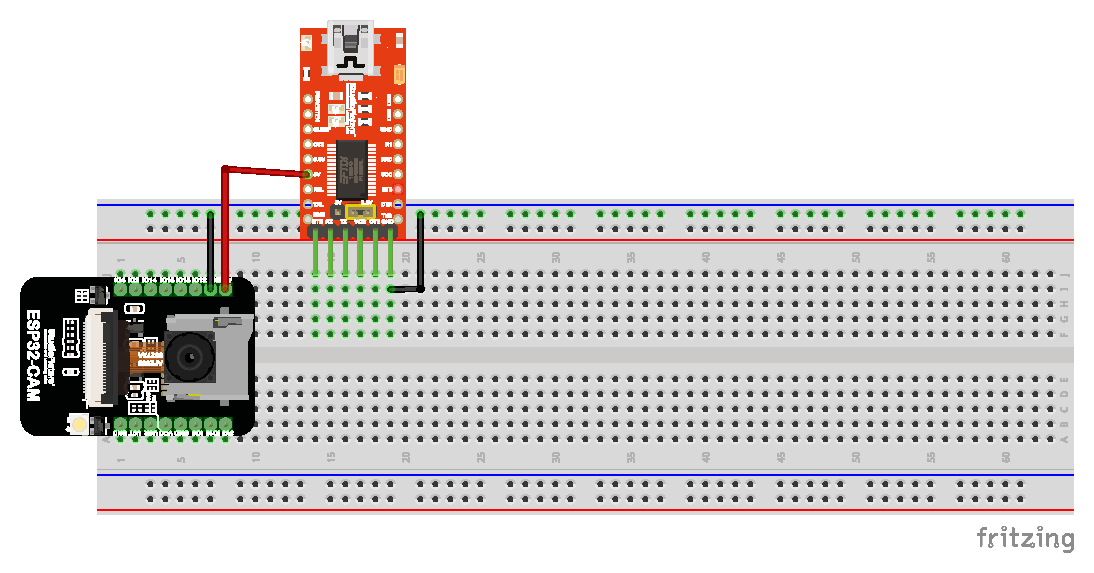
\includegraphics[width=16cm]{./img/ESP32 CAM schematics}
		\caption{\Az{\textsc{ESP32-CAM}} bekötése}
		\label{esp32-cam-schematics}
	\end{figure}	
	
	\subsection{DHT22 - hőmérséklet és páratartalom szenzor}
	
	Az DHT22 érzékelő egy olyan eszköz, amely méri a levegő hőmérsékletét és a relatív  páratartalmát. Az összegyűjtött adatokat feldolgozza és továbbítja. A DHT22 kis mérete, alacsony energiafogyasztása miatt széles körben használható különböző alkalmazásokban.\cite{dht22}
	
	Ebben a rendszerben úgy van alkalmazva, hogy egy ESP-WROOM-32-höz van kapcsolva, és ez 10 másodpercenként elküldi az adatokat a webalkalmazásnak, mely eltárolja az adott pillanatban mért adatokat az alkalmazott szobában, és jeleníti meg a főoldalon, mely alapján meg lehet tekinteni az elmúlt 24 órai adatokat egy grafikonon is.\footref{later-expl-fn}
		\begin{figure}[ht!]
		\centering
		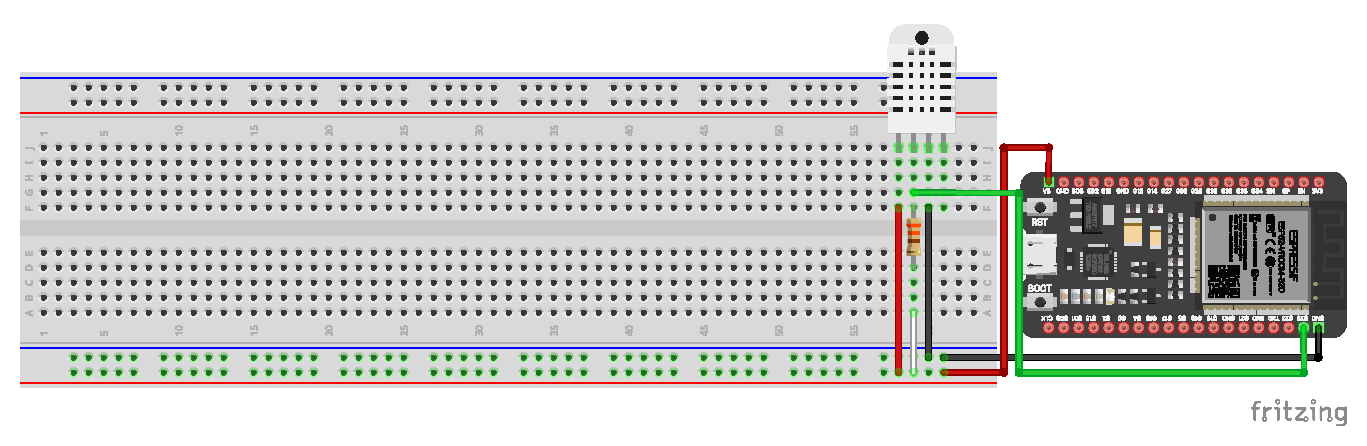
\includegraphics[width=16cm]{./img/temperature and humidity sensor_bb}
		\caption{\Az{\textsc{ESP-WROOM-32}} bekötése DHT22 hőmérséklet és páratartalom szenzorral}
		\label{dht22-schematics}
	\end{figure}	
	
	\subsection{Mi is az RFID?}\label{what-is-rfid}
	A Radio Frequency Identification\footnote{Magyarul: rádiófrekvenciás azonosítás} (RFID) olyan vezeték nélküli rendszer, amely két összetevőből áll: tag-ekből\footnote{Magyarul: címkékből} és olvasókból. Az olvasó egy olyan eszköz, amely olyan antennával rendelkezik, ami rádióhullámokat bocsát ki, és jeleket fogad vissza az RFID-tag-ről. A tag-ek lehetnek passzívak vagy aktívak. A passzív RFID-címkéket az olvasó táplálja, és nincs sajét áramforrásuk. Az aktív RFID címkék akkumulátorral, vagy hálózatról működnek.
	
	Az RFID-címkék számos információt tárolhatnak egy azonosítótól több oldalnyi adatig. Az olvasók lehetnek mozgathatóak, így kézben is hordhatók, vagy oszlopra vagy falra is rögzíthetőek. Egy olvasó egy szekrény, szoba vagy épület architektúrájába is beépíthető.\cite{rfid-desc}
	
	\subsection{RFID-RC522 - RFID olvasó}
	Mint ahogyan \aref{what-is-rfid}~. szakaszban említve lett, ez egy RFID olvasó, amely képes RFID tag-eknek az azonosítójukat, és egyéb adatait beolvasni rádióhullámok alkalmazásával.
	
	A rendszerben úgy van jelen, mint egy kezdetleges ,,biztonsági rendszer'', amit például ajtóknak, vagy szekrényeknek zárására lehetne használni. Jelen esetben úgy van alkalmazva, hogy az RFID olvasót működtető ESP-WROOM-32 elküldi a Raspberry Pi számára az adott tag adatait: hogy, ha ez megegyezik az adatbázisban jelen levő azonosító egyikével, akkor -- jelenlegi rendszerben -- az RGB LED\footnote{\label{rgb-led}Red Green Blue Light Emitting Diode, magyarul Piros Zöld Kék Fényt Kibocsátó Dióda} zölden kezd villogni, ellenkező esetben pedig pirosan fog villogni.\footref{later-expl-fn}
	
	\begin{figure}[ht!]
		\centering
		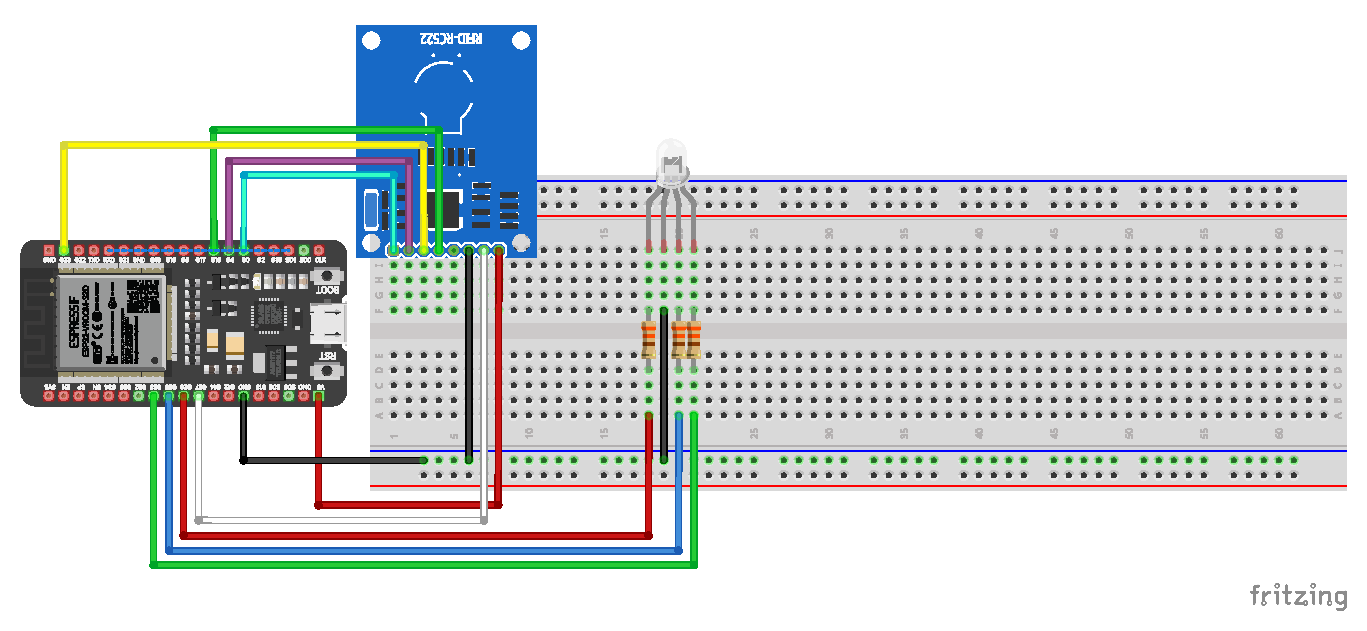
\includegraphics[width=16cm]{./img/RFID reader schematics_bb}
		\caption{\Az{\textsc{ESP-WROOM-32}} bekötése, RFID-RC522 olvasóval és egy RGB LED-del}
		\label{rfid-schematics}
	\end{figure}	
	
	\subsection{Szilárdtest relé}
	
	A szilárdtest relé az egy elektronikus kapcsolóeszköz. Az elektromechanikus reléhez hasonlóan képes be- vagy kikapcsolni az átfolyó áramot, ha külső vezérlőjelet adnak át a vezérlőn. Az elektromechanikus reléhez képest a szilárdtest relék azonban nem tartalmaznak mozgó alkatrészeket, ezért nem hangosak és hosszabb életűek. 
	
	A félvezetők elektromos és optikai tulajdonságait használják fel a kapcsolás végrehajtására, és teljes leválasztást biztosítanak a vezérlőáramkör és a terhelési áramkör között.\cite{solid-state-relay}
	
	Ebben a rendszerben úgy lett alkalmazva ez, hogy egy ESP-WROOM-32 és egy izzó van csatlakoztatva egy szilárdtest reléhez. Az ESP-WROOM-32 rákapcsolódva a Raspberry Pi-ra képes azt a felhasználó a felületen keresztül ki- vagy bekapcsolni.\footref{later-expl-fn}
	
	De akár számos más olyan eszközt lehet ezzel alkalmazni, amit ki- vagy be lehetne kapcsolni: mint például egy ventilátor.
	
	\begin{figure}[ht!]
		\centering
		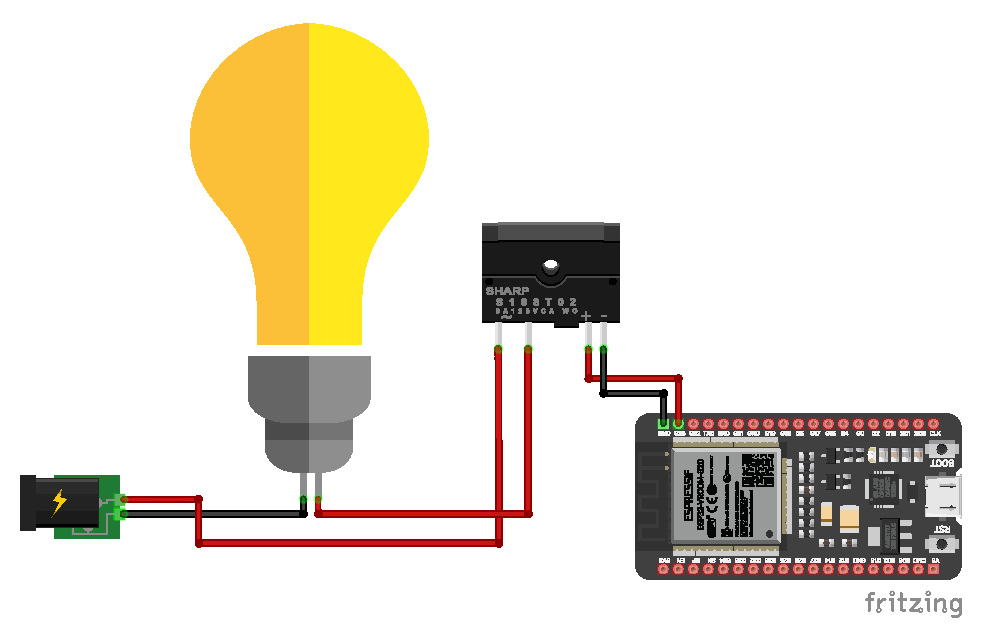
\includegraphics[width=16cm]{./img/ESP32 toggle schematics_bb}
		\caption{\Az{\textsc{ESP-WROOM-32}} bekötése szolidtest-relével és egy izzóval}
		\label{toggle-schematics}
	\end{figure}	
	
	%----------
	\section{Szoftverek és Programozási nyelvek}
	\subsection{C++ és Arduino IDE}
	A Bjarne Stroustrup által 1979-ben lett kifejlesztve a C++, ami egy általános célú programozási nyelv, ami lényegében a C programozási nyelv továbbfejlesztett változata. A főbb kiegészítések közé tartozott az objektumorientált programozás, és a hiba- és végrehajtás kezelés.\cite{cpp}
	
	A mikrokontrollerek legtöbbjét C++-al szokták programozni, amihez az Arduino IDE az egyik legnépszerűbb választás, ami számos kiegészítőkkel, és mikrokontrollerek programozásához használatos funkciókkal rendelkezik, legyen ez a kód feltöltése, vagy a soros monitorra kiírt információk kiírása. Külső könyvtárak is hozzáadhatóak a különböző eszközök támogatása érdekében. 
	
	\subsection{HTML és CSS}
	A HTML\footnote{Azaz Hyper Text Markup Language ami magyarul Hiper Szöveg Leíró Nyelv}  egy leírónyelv, amely szövegek leírására és megjelenítésére szolgál. Számos funkciója van ennek, mint a bekezdések, táblázatok, vagy képek beszúrása. Ezt legtöbbnyire weboldalak elkészítésénél használják. Mezőket ,,<>''-en belül határozzuk meg és lezárni ehhez hasonlóan ,,</>''-el kell. Mindezt annak megfelelően kell párosítani, hogy mit is írunk: legyez ez például egy bekezdés, ami ,,<p>\footnote{azért ,,p'' a bekezdés, mert angolul ez a szó úgy van, hogy paragraph} </p>'' aminek a két tag közé kell beírni a szöveget.
	
	Mindez kevés arra, hogy a szöveg kinézetét változtassuk, ezért is társítják melléje a CSS-t, azaz Cascading Style Sheet-et\footnote{Magyarul: Kaszkádolt Stílus Lap}, ami HTML vagy XML nyelvek által meghatározott megjelenés formázására szolgál. Ezeket a stílus leírásokat ,,<style></style>'' tag-ek közé szoktuk leírni. Megvan ennek is a sajátos meghatározási módja, hogy mit- és hogyan alkalmazunk.
	
	A webalkalmazásnál máshogyan állítom be a kinézetet, amit \aref{tailwind} részen említek, hogy hogyan is működik a Tailwind.
	
	\subsection{PHP}
	A PHP \footnote{PHP: Hypertext Preprocessor, magyarul: PHP: hiperszöveg előfeldolgozó} egy általános felhasználású szkriptnyelv, és fordító, amely szabadon elérhető és széles körben használt webfejlesztés során. A nyelvet elsősorban szerveroldali szkriptek készítésére használják, bár használható parancssori szkriptekre is, és korlátozott mértékben alkalmazásokra.\cite{php}
	
	C programozási nyelv jellegű a szintaxisa, és rendkívül engedékeny programozási nyelv. Amikor PHP-ban akarunk valamit írni, akkor azt .php-re végződő fájlban írjuk, aminek a belső tartalma ,,<?php''-vel kezdődik, és ,,?>''-vel végződik. Ezek között írható le a kódunk. Legtöbb esetben HTML-el van társítva.
	
	\subsection{JavaScript}
	A JavaScript az egy objektum orientált programozási nyelv, ami elsősorban interaktív elemek létrehozására van használva weboldalakon vagy alkalmazásokon, azonban ez átterjedt sok más környezetre és használati területre is.
	
	A JavaScript megtanulása és futtatása felettébb egyszerű, és rendkívül híres és gyakran használt programozási nyelv.\cite{javascript}
	
	A webalkalmazásomban is a felületen sok helyen JavaScript-et, azon belül is a jQuery-t használom funkciók kezelésére, legyen az például egy lámpa felkapcsolásának kezdeményezése.\footref{later-expl-fn}
	
	\subsection{jQuery}
	A jQuery az egy ingyenes és nyílt forráskódú, gyors, kisméretű és funkciókban gazdag JavaScript könyvtár. Sokkal egyszerűbbé teszi az olyan dolgokat, mint a HTML elemek elérése és kezelése, az eseménykezelés, és az animáció egy könnyen használható API-val, amely számos böngészőben működik. A sokoldalúság és a bővíthetőség kombinációjával a jQuery emberek millióinak JavaScript-írási módját változtatta meg. \cite{jquery}
	
	\subsection{Chart.js}
	Chart.js egy népszerű, nyílt forráskódú JavaScript könyvtár, amely lehetővé teszi a fejlesztők számára, hogy könnyen létrehozzanak reszponzív és testre szabható diagramokat vagy grafikonokat a weben. Többféle diagram típust támogat.
	
	A könyvtár a HTML5-re épül, amely lehetővé teszi a gördülékeny animációkat és az interaktivitást. A Chart.js egy egyszerű API-t kínál, amely lehetővé teszi a fejlesztők számára a diagramok egyszerű beállítását és stílusának testreszabását. Több beépített testreszabási lehetőséget is biztosít, mint például a diagramszínek, címkék, és jelmagyarázatok.\cite{chartJS}
	
	Chart.js nagy előnye, hogy a hivatalos oldalukon részletesen le van dokumentálva, hogy hogyan kell telepíteni, és mit hogyan is lehet használni, példákon keresztül.
	
	A Chart.js a egy adott szobában lévő hőmérséklet és páratartalom szenzor adatok grafikonon való megjelenítésére volt használva a weboldalon.
	
	\subsection{Tailwind CSS}\label{tailwind}
	A Tailwind CSS egy népszerű CSS keretrendszer, amely előre definiált osztályokat biztosít a webalkalmazások stílusának egyszerűsítéséhez és optimalizálásához. Ezek olyan osztályok formájában vannak meghatározva, amik leírják a kívánt vizuális hatást, ahelyett, hogy egyedi CSS stílusokat írnának az egyes elemekre.\footnote{Mindezt build-elés, azaz felépítés idejében átalakítja CSS kóddá, és a felesleges elemeket kihagyja.}
	
	Például egy bekezdéshez így tudjuk azt megadni azt, hogy a szövege jobbra zárt és félkövér legyen: \emph{<p \textbf{class="text-right font-bold"}\footnote{text-right, azaz szöveg-jobb, font-bold, azaz szöveg-félkövér}> ez egy bekezdés </p>}
	
	A Tailwind stílus alkalmazása lehetővé teszi a fejlesztők számára a gyors, összehangolt és egységes felület létrehozását, miközben javítja a kinézet gyors alakíthatóságát és skálázhatóságát, azonban ezzel rontva a HTML fájl átláthatóságát.
	
	Széles választékban kínál előre elkészített osztályokat a közös UI\footnote{User Inerface: azaz Felhasználói Felület} komponensekhez egy konfigurációs fájlban, mint például gombok, űrlapok, grid rendszerek és tipográfiák, valamint a bonyolultabb elrendezésekhez és pozicionálási feladatokhoz is. Ezzel a konfigurációs fájlal biztosítja a fejlesztőknek, hogy a beépített osztályokat testre szabhassák és, hogy saját egyedi osztályokat is létre hozhassanak. 
	
	Fejlesztést pedig hivatalos dokumentációval segítik, mivel mindenre van nekik példa és leírás.\cite{tailwind-docs}
	
	
	\subsection{dbDiagram.io}
	A dbdiagram.io egy webes eszköz, amely lehetővé teszi a felhasználók számára az adatbázis tervek létrehozását egy letisztult vizuális felületen keresztül. 
	
	Az eszköz támogatja különböző adatbázis rendszereket, mint például a MySQL. Hasznos funkciókat kínál, mint például az automatikus SQL kódgenerálás, és a diagramok importálása vagy exportálása különböző formátumokba.\cite{dbdiagram-io}
	
	Szakdolgozatom során ez volt használva arra, hogy elkészítsem az adatbázis tervét, és majd \aref{database} szakaszon lesz róla egy mellékelt kép is, hogy hogyan is lett mindez kialakítva.
	
	\subsection{Font Awesome}
	A Font Awesome egy népszerű nyílt forráskódú ikon könyvtár, amely skálázható vektor ikonokat\footnote{Ez azt jelenti, hogy egy algoritmus segítségével mindig ugyan olyan minőségű lesz a kép, bármekkorára is nagyítjuk.}kínál, amelyek testre szabhatóak az oldalukon, és CSS alkalmazásával is. A könyvtár több ezer ikont tartalmaz, amik széles körű kategóriákat fednek le, például márka vagy közösségi média ikonokat. Lehetőség van fizetős és ingyenes ikonok használatára is.
	
	A Font Awesome egy rugalmas és könnyen használható megoldást kínál az ikonok hozzáadásához weboldalakhoz vagy alkalmazásokhoz, lehetővé téve a fejlesztőknek, hogy feldobják projektjeik kinézetét. A könyvtár folyamatosan frissül új ikonokkal és funkciókkal.\cite{fontawesome}\\
	\textbf{Az általam használt ikonok, a rendszerben:}
	\begin{itemize}
		\item 
\includegraphics[width=0.5cm]{./img/arrow-left-solid}
		 	\emph{,,<i class="fa-solid fa-arrow-left"></i>''}
		
		\item 
\includegraphics[width=0.5cm]{./img/clock-rotate-left-solid} 
			\emph{,,<i class="fa-solid fa-clock-rotate-left"></i>''}
			
		\item 
\includegraphics[width=0.5cm]{./img/plus-solid} 
			\emph{,,<i class="fa-solid fa-plus"></i>''}
		
		\item 
\includegraphics[width=0.5cm]{./img/pen-to-square-regular}
			\emph{,,<i class="fa-regular fa-pen-to-square"></i>''}
			
		\item 
\includegraphics[width=0.5cm]{./img/trash-can-solid}
			\emph{,,<i class="fa-solid fa-trash-can"></i>''}
			
		\item 
\includegraphics[width=0.5cm]{./img/arrow-rotate-right-solid}
			\emph{,,<i class="fa-solid fa-rotate-right"></i>''}
		
		\item 
\includegraphics[width=0.5cm]{./img/ban-solid}
		 	\emph{,,<i class="fa-solid fa-ban"></i>''}
			
		\item 
\includegraphics[width=0.5cm]{./img/gear-solid}
			\emph{,,<i class="fa-solid fa-gear"></i>''}
			
		\item 
\includegraphics[width=0.5cm]{./img/key-solid}
			\emph{,,<i class="fa-solid fa-key"></i>''}
			
		\item 
\includegraphics[width=0.5cm]{./img/id-card-clip-solid}
			\emph{,,<i class="fa-solid fa-id-card-clip"></i>''}
			
	\end{itemize}
	\subsection{MySQL}
	A MySQL egy nyílt forráskódú adatbázis-kezelő rendszer, amelyet széles körben használnak webalkalmazásokhoz. Lehetővé teszi a felhasználók számára, hogy relációs adatbázisokat hozzanak létre, kezeljenek és tartsanak karban. Több platformon is működik és sok programozási nyelvvel is kompatibilis.
	
	A XAMPP egy webszerver szoftver, amely tartalmazza a MySQL adatbázis-kezelő rendszert, és a PHP-t is, a,o telepíthető a helyi számítógépre webfejlesztéshez és teszteléshez, mint ahogyan én is alkalmaztam lokális fejlesztés során.
	\subsection{PlantUML}
	A PlantUML egy ingyenes és nyílt forráskódú eszköz, amely egyszerű szövegszintaxist használ a különböző formátumokban létrehozott UML\footnote{Unified Modeling Language, magyarul Egységesített Modellező Nyelv} diagramok készítéséhez. Többféle diagramtípus támogatása mellett használható szoftverfejlesztéshez és rendszertervezéshez.

	Ennek segítségével rajzoltam le azt, hogy NodeMCU és a Raspberry Pi hogyan is kommunikál a rendszeren belül.\footref{later-expl-fn}
	\subsection{Fritzing}
	A Fritzing az egy nyílt forráskódú szoftver, aminek a segítségével elektronikai eszközök kötési és sematikus rajzait, de akár szimulációt is lehet benne készíteni.
	
	Ez egy olyan program, aminek a letöltéséért cserébe fizetni kell, ezzel is támogatva a program fejlesztését és karbantartását. Letölthetőek hozzá külső könyvtárak, ezzel is növelve a lehetőségeket ilyen rajzok létrehozásában.
	
	Ennek használatával hoztam létre \aref{hardware-sec}~.szakaszban a kötési rajzokat.\\
	\textbf{Külső könyvtárak, amik voltak használva a rajzokban:}
	\begin{itemize}
		\item \Aref{esp32-cam-schematics}.~ábrán az ESP-WROOM-32, az ESP32-CAM, és az FTDI Adapter\cite{fritzing-library}
		\item \Aref{dht22-schematics}.~ábrán az ESP-WROOM-32 és a DHT22 szenzor \cite{fritzing-library}
		\item \Aref{rfid-schematics}.~ábrán az ESP-WROOM-32\cite{fritzing-library} és az RFID-RC522\cite{fritzing-rfid}
		\item \Aref{toggle-schematics}.~ábrán az ESP-WROOM-32\cite{fritzing-library} az izzó\cite{fritzing-light} és a szilárdtest relé\cite{fritzing-SSR}
	\end{itemize}
	\subsection{Laravel}
	A Laravel egy ingyenes és nyílt forrású PHP webalkalmazás-keretrendszer, amelyet skálázható és nagy méretű webalkalmazások építésére használnak. Egy elegáns szintaxist, erős eszközöket és moduláris csomagolási rendszert biztosít, hogy a fejlesztők tiszta és karbantartható kódot írhassanak. A Laravel követi az MVC\footnote{Model-View-Controller: magyarul Modell-Nézet-Vezérlő} architekturális mintát, és beépített funkciókkal rendelkezik, mint például az azonosítás, a route-olás és gyorsítótár.\cite{laravel-intro}
	A fejlesztők dolgát azzal könnyítik meg leginkább, hogy hivatalos dokumentációja van, ahol minden kis részletre adnak példát és leírást.\cite{laravel-docs}\\
	\textbf{MVC Keretrendszer}:\\
	Az MVC az egy szoftvertervezési minta, amelyet a felhasználói felületek fejlesztéséhez használnak. \\
	\textbf{Az alkalmazást három összekapcsolt komponensre bontja}:\\A \textbf{modell}, amely az adatokat és a logikát képviseli, a \textbf{nézet}, amely megjeleníti az adatokat a felhasználónak, és a \textbf{vezérlő}, amely kezeli a felhasználói bemenetet és kapcsolatban áll a modellel és a nézettel. Az MVC keretrendszerek, mint például a Laravel, strukturált megközelítést biztosítanak a webalkalmazások fejlesztéséhez, és segítik a fejlesztőket a moduláris és karbantartható kód írásában.
	
	Éppen ezért is esett a választásom a projekt tervezési fázisában a Laravel keretrendszerre. Ez a webalkalmazás még Laravel 9-nél indult el.
	
	\chapter{A web alkalmazás felépítése és működése}
	\section{Raspberry PI4B alkalmazása, mint Wi-Fi, és hub}
	\section{Adatbázis felépítése}\label{database}
	%----------
	\section{Kezelő felület bemutatása és működése}
	\subsection{Főoldal}
	\subsection{Beállítások}
	\subsection{RFID beállítások}
	\subsection{RFID használati táblázat}
	\subsection{Hőmérsékleti és páratartalom előzmények - ChartJS}
	%----------
	\section{Eszközök kommunikációja a webszerverrel}\label{csatlakozas-a-webszerverre}
	\subsection{Hőmérséklet és Páratartalom szenzor}
	\subsection{Eszköz kapcsoló}
	\subsection{Kamera}
	\subsection{RFID kártya olvasó}
	
	%----------
	
	\chapter{Tesztelések}
	\section{Tesztelések módjai és fontossága}
	
	\subsection{Cypress automatizált tesztelések}
	\subsection{Manuális tesztelések}
	\begin{table}[ht]
		\centering
		\begin{tabular}{|p{6cm}|p{6cm}|p{4cm}|}
			\hline
			\textbf{Teszt leírása} & \textbf{Elvárt eredmények} & \textbf{Tapasztalatok} \\
			\hline
			Access Control Test: RFID tags assigned to users &
			 The system should recognize the RFID tags assigned to each user and grant or deny access to specific devices or areas of the home accordingly &
			  The test was successful, with the system accurately recognizing and responding to each user's assigned RFID tag \\
			\hline
			Device Control Test: Using RFID tags to control devices &
			 The system should allow users to control smart home devices (such as lights or locks) using RFID tags, without requiring additional input &
			  The test was partially successful, with the system accurately recognizing the RFID tags but experiencing some delays in device response times \\
			\hline
			Durability Test: RFID tags in high traffic areas &
			 The RFID tags should remain functional and readable even in high traffic areas, with no degradation in performance &
			  The test was successful, with the RFID tags remaining fully functional and readable even with heavy usage \\
			\hline
			Security Test: Unauthorized access prevention &
			 The system should be designed to prevent unauthorized access by detecting and alerting the user to the presence of unrecognized RFID tags & 
			 The test was successful, with the system detecting and preventing access by an unrecognized RFID tag, and sending an alert to the user's mobile device \\
			\hline
		\end{tabular}
		\caption{Manuális tesztelések a webalkalmazásra}
		\label{table:manual-testing-results}
	\end{table}
	
	%----------
	\chapter{Rendszer telepítése}

	
	\chapter*{Összegzés}
	\addcontentsline{toc}{chapter}{Összegzés}
	
	\begin{thebibliography}{20}
		\addcontentsline{toc}{chapter}{\bibname}
		
		\bibitem{amazon-api}
		\textsc{Jeff Blankenburg}: \emph{Define Your Appliance Category for a Better Customer Experience}\\
		\textsc{URL:}%
		 \url{https://developer.amazon.com/blogs/alexa/post/a89f7243-08a0-4c73-8fc5-eb604a93f437/define-your-appliance-category-for-a-better-customer-experience}\\
		\textsc{Link utoljára ellenőrizve:} 2023.03.31.
		
		\bibitem{amazon-stats}
		\textsc{Jason Wise}: \emph{How Many People Use Alexa in 2023? (U.S. Amazon Statistics)} \\
		\textsc{URL:} \url{https://earthweb.com/alexa-users/}\\
		\textsc{Link utoljára ellenőrizve:} 2023.03.31.
		
		\bibitem{xiaomi-home}
		\textsc{HandWiki}: \emph{Engineering:Xiaomi Smart Home}
		\textsc{URL:} \url{https://handwiki.org/wiki/Engineering:Xiaomi_Smart_Home}\\
		\textsc{Link utoljára ellenőrizve:} 2023.03.31.
		
		\bibitem{what-is-open-source}
		\textsc{What is open source}\\
		\textsc{URL:} \url{https://opensource.com/resources/what-open-source}\\
		\textsc{Link utoljára ellenőrizve:} 2023.03.31.
		
		\bibitem{creation-of-home-assistant}
		\textsc{Eric Brown}: \emph{Home Assistant: The Python Approach to Home Automation}\\
		\textsc{URL:} \url{https://www.linux.com/topic/embedded-iot/home-assistant-python-approach-home-automation/}\\
		\textsc{Link utoljára ellenőrizve:} 2023.03.31.
		
		\bibitem{home-assistance-itegrations}
		\textsc{Home Assistant - Integrations}\\
		\textsc{URL:} \url{https://www.home-assistant.io/integrations/}\\
		\textsc{Link utoljára ellenőrizve:} 2023.03.31.
		
		\bibitem{openhab}
		\textsc{OpenHAB hivatalos oldala}\\
		\textsc{URL:} \url{https://www.openhab.org/}\\
		\textsc{Link utoljára ellenőrizve:} 2023.03.31.
		
		\bibitem{raspberrypi-history}
		\textsc{The Epic Story of the Raspberry Pi}\\
		\textsc{URL:} \url{https://raspberrytips.com/raspberry-pi-history/}\\
		\textsc{Link utoljára ellenőrizve:} 2023.03.31.
		
		\bibitem{raspberrypi-4b}
		\textsc{Offical Raspberry Pi 4B dokumentation}\\
		\textsc{URL:} \url{https://www.raspberrypi.com/documentation/computers/raspberry-pi.html#raspberry-pi-4}\\
		\textsc{Link utoljára ellenőrizve:} 2023.03.31.
		
		\bibitem{esp-32-datasheet}
		\textsc{Espressif Systems:} \emph{ESP32­-WROOM-­32 Datasheet}\\
		\textsc{URL:} \url{https://www.espressif.com/sites/default/files/documentation/esp32-wroom-32_datasheet_en.pdf}\\
		\textsc{Link utoljára ellenőrizve:} 2023.03.31.
		
		\bibitem{esp32-devices}
		\textsc{Offical ESP32 devices documentation}\\
		\textsc{URL:} \url{http://esp32.net/#Info}\\
		\textsc{Link utoljára ellenőrizve:} 2023.03.31.
		
		\bibitem{esp-8266}
		\textsc{ANAT ZAIT:} \emph{NODEMCU - A PERFECT BOARD FOR IOT}\\
		\textsc{URL:} \url{https://www.circuito.io/blog/nodemcu-esp8266/}\\
		\textsc{Link utoljára ellenőrizve:} 2023.03.31.
		
		\bibitem{dht22}
		\textsc{Aosong Electronics Co.,Ltd:} \emph{Digital-output relative humidity \& temperature sensor/module DHT22 (DHT22 also named as AM2302)}\\
		\textsc{URL:} \url{https://www.sparkfun.com/datasheets/Sensors/Temperature/DHT22.pdf}\\
		\textsc{Link utoljára ellenőrizve:} 2023.03.31.
		
		\bibitem{rfid-desc}
		\textsc{U.S. Food and Drug Administration:} \emph{Radio Frequency Identification (RFID)}\\
		\textsc{URL:} \url{https://www.fda.gov/radiation-emitting-products/electromagnetic-compatibility-emc/radio-frequency-identification-rfid}\\
		\textsc{Link utoljára ellenőrizve:} 2023.03.31.
		
		\bibitem{rfid-datasheet}
		\textsc{Handson Technology:} \emph{RC522 RFID Development Kit}\\
		\textsc{URL:} \url{http://www.handsontec.com/dataspecs/RC522.pdf}\\
		\textsc{Link utoljára ellenőrizve:} 2023.03.31.
		
		\bibitem{solid-state-relay}
		\textsc{Jayesh Upadhyay:} \emph{How do Solid State Relays work?}\\
		\textsc{URL:} \url{https://www.circuitbread.com/ee-faq/how-do-solid-state-relays-work}\\
		\textsc{Link utoljára ellenőrizve:} 2023.03.31.
		
		\bibitem{cpp}
		\textsc{Romain Juillet:} \emph{Essentials of Programming in C++}\\
		\textsc{URL:} \url{https://www.bocasay.com/essentials-programming-c/}\\
		\textsc{Link utoljára ellenőrizve:} 2023.03.31.
		
		\bibitem{php}
		\textsc{Robert Sheldon:} \emph{DEFINITION: PHP (Hypertext Preprocessor)}\\
		\textsc{URL:} \url{https://www.techtarget.com/whatis/definition/PHP-Hypertext-Preprocessor}\\
		\textsc{Link utoljára ellenőrizve:} 2023.03.31.
		
		\bibitem{javascript}
		\textsc{Susan Simkins:} \emph{Quick Start to JavaScript: Volume 1}\\
		\textsc{URL:} \url{https://www.pluralsight.com/courses/quick-start-javascript-1-1870}\\
		\textsc{Link utoljára ellenőrizve:} 2023.03.31.
		
		\bibitem{jquery}
		\textsc{jQuery}\\
		\textsc{URL:} \url{https://jquery.com/}\\
		\textsc{Link utoljára ellenőrizve:} 2023.03.31.
		
		\bibitem{chartJS}
		\textsc{Chart.js hivatalos dokumentáció oldala}\\
		\textsc{URL:} \url{https://www.chartjs.org/docs/latest/}\\
		\textsc{Link utoljára ellenőrizve:} 2023.03.31.
		
		\bibitem{tailwind-docs}
		\textsc{Tailwind CSS hivatalos dokumentáció oldala}\\
		\textsc{URL:} \url{https://tailwindcss.com/docs}\\
		\textsc{Link utoljára ellenőrizve:} 2023.03.31.
		
		\bibitem{dbdiagram-io}
		\textsc{dbDiagram.io oldala}\\
		\textsc{URL:} \url{https://dbdiagram.io/home}\\
		\textsc{Link utoljára ellenőrizve:} 2023.03.31.
		
		\bibitem{fontawesome}
		\textsc{Fontawesome - Free Icons}\\
		\textsc{URL:} \url{https://fontawesome.com/search?o=r&m=free}\\
		\textsc{Link utoljára ellenőrizve:} 2023.03.31.
		
		\bibitem{fritzing-library}
		\textsc{Achim Pieters} \emph{Fritzing – New Parts}\\
		\textsc{URL:} \url{https://www.studiopieters.nl/fritzing/}\\
		\textsc{Link utoljára ellenőrizve:} 2023.03.31.
		
		\bibitem{fritzing-light}
		\textsc{Alfred Dagenais} \emph{Fritzing Components - Light bulb}\\
		\textsc{URL:} \url{https://github.com/alfreddagenais/fritzing-components/}\\
		\textsc{Link utoljára ellenőrizve:} 2023.03.31.
		
		\bibitem{fritzing-SSR}
		\textsc{Fritzing Forum} \emph{SSR-40va solid state relay}\\
		\textsc{URL:} \url{https://forum.fritzing.org/t/ssr-40va-solid-state-relay/16832}\\
		\textsc{Link utoljára ellenőrizve:} 2023.03.31.
		
		\bibitem{fritzing-rfid}
		\textsc{amontanes} \emph{RFID-RC522}\\
		\textsc{URL:} \url{https://fritzing.org/projects/mfrc522}\\
		\textsc{Link utoljára ellenőrizve:} 2023.03.31.
		
		\bibitem{laravel-intro}
		\textsc{Laravel - Overview}\\
		\textsc{URL:} \url{https://www.tutorialspoint.com/laravel/laravel_overview.htm}\\
		\textsc{Link utoljára ellenőrizve:} 2023.03.31.
		
		\bibitem{laravel-docs}
		\textsc{Offical Laravel Documentation}\\
		\textsc{URL:} \url{https://laravel.com/docs/10.x}\\
		\textsc{Link utoljára ellenőrizve:} 2023.03.31.
		
		\bibitem{RFID-card-reader}
		\textsc{Connect RFID to PHP \& MySQL Database with NodeMcu ESP8266}\\
		\textsc{URL:} \url{https://iotprojectsideas.com/connect-rfid-to-php-mysql-database-with-nodemcu-esp8266/}\\
		\textsc{Link utoljára ellenőrizve:} 2023.03.31.
		
		\bibitem{node32-httpget}
		\textsc{ESP8266 NodeMCU HTTP GET and HTTP POST with Arduino IDE (JSON, URL Encoded, Text)}\\
		\textsc{URL:} \url{https://randomnerdtutorials.com/esp8266-nodemcu-http-get-post-arduino/#http-get-1}\\
		\textsc{Link utoljára ellenőrizve:} 2023.03.31.
		
		\bibitem{arduino-to-laravel}
		\textsc{Arduino to Laravel Communication}\\
		\textsc{URL:} \url{https://www.instructables.com/Arduino-to-Laravel-Communication/}\\
		\textsc{Link utoljára ellenőrizve:} 2023.03.31.
		
		\bibitem{raspberry-as-wifi}
		\textsc{Raspberry configuration for Wi-Fi}\\
		\textsc{URL:} \url{https://www.raspberrypi.com/documentation//computers/configuration.html#setting-up-a-routed-wireless-access-point}\\
		\textsc{Link utoljára ellenőrizve:} 2023.03.31.
	
		\bibitem{cypress-docs}
		\textsc{Offical Cypress Documentation}\\
		\textsc{URL:} \url{https://docs.cypress.io/guides/overview/why-cypress}\\
		\textsc{Link utoljára ellenőrizve:} 2023.03.31.
				
	\end{thebibliography}
	
	% Aláírt, szkennelt nyilatkozat beillesztése a szakdolgozat végére
	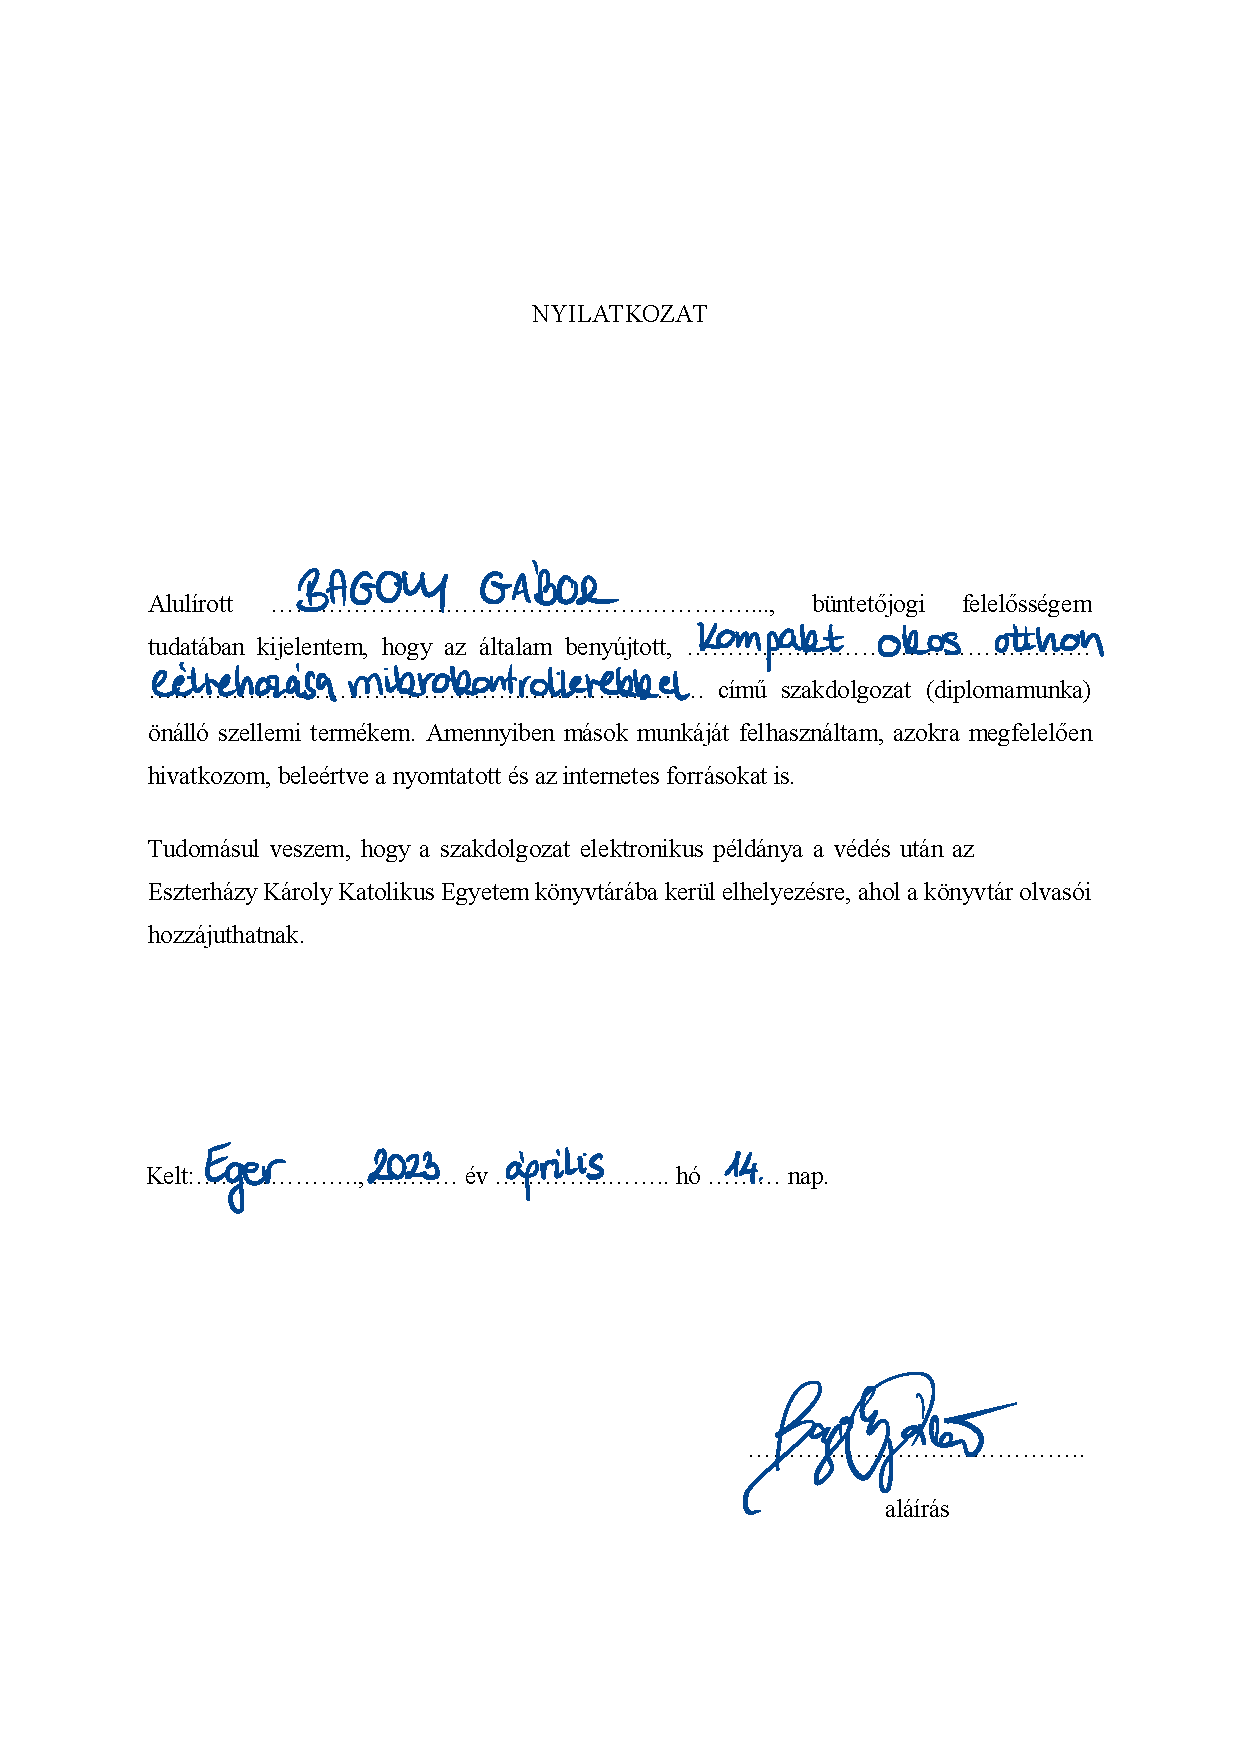
\includepdf{nyilatkozat.pdf}
\end{document}